\documentclass{article}

\usepackage{graphicx}
\usepackage{tikz}
\usepackage{tikzsymbols}
\usetikzlibrary{calc,patterns,shapes.geometric}
\pagestyle{empty}
\usepackage[margin=0pt]{geometry}
\geometry{papersize={14in,12in}}

\def\centerarc[#1](#2)(#3:#4:#5){\draw[#1] ($(#2)+({#5*cos(#3)},{#5*sin(#3)})$) arc (#3:#4:#5);}

\begin{document}
	\begin{figure}
		\centering
		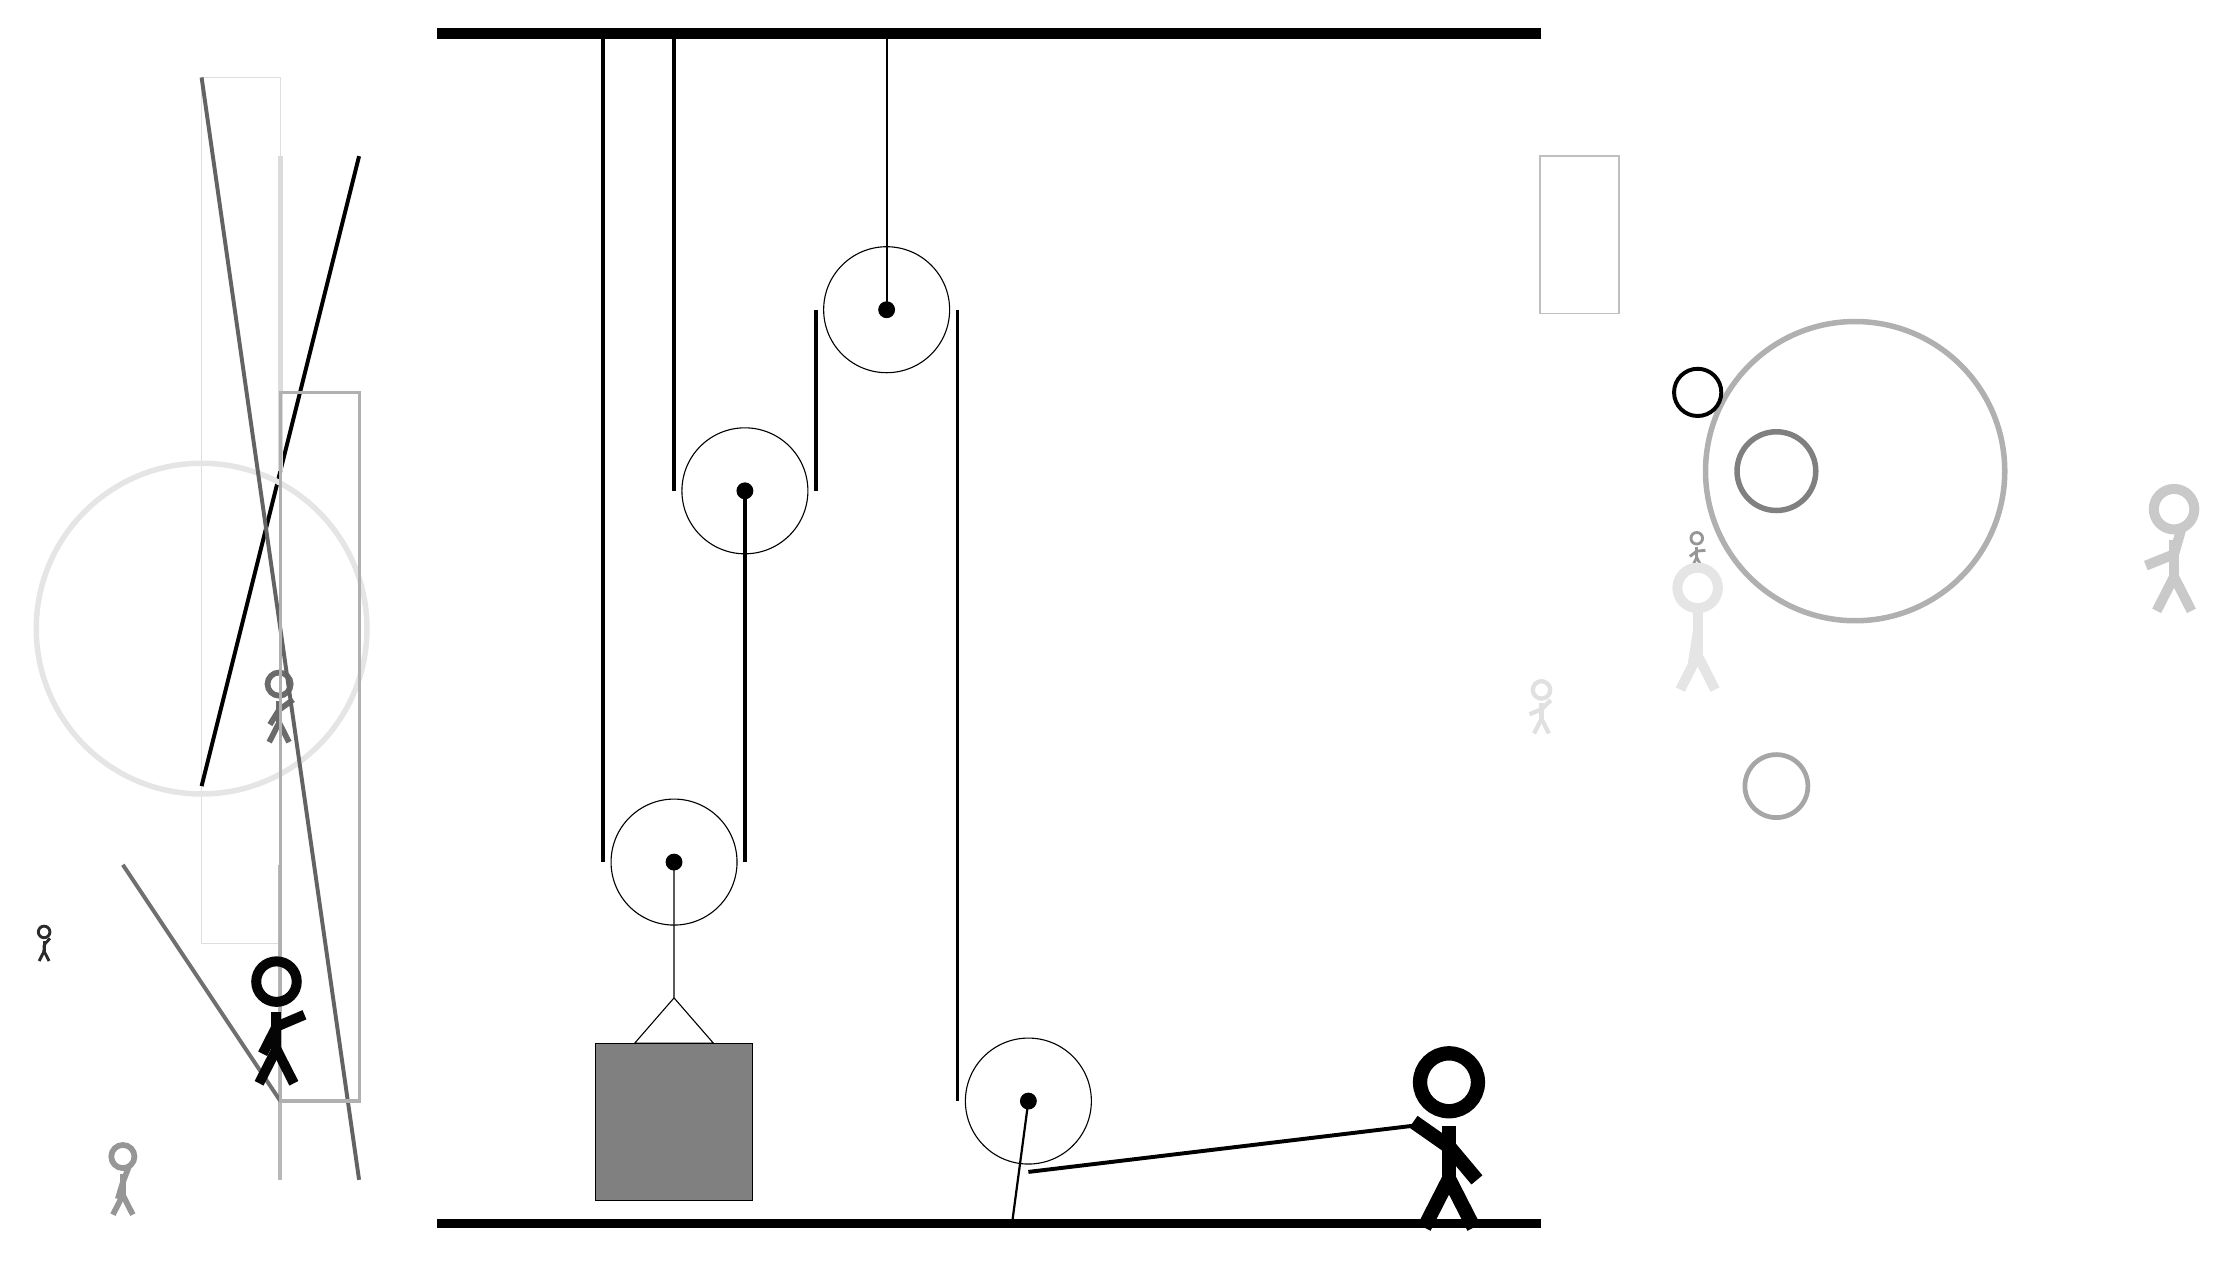
\begin{tikzpicture}
			%%%%% START %%%%%
			
			\draw[fill=black] (-2, 11.5) rectangle (12, 11.625);
			
			\draw (1, 1.035) circle (0.8);
			\draw[fill=black] (1, 1.035) circle (0.1);
			
			\draw (1.9, 5.75) circle (0.8);
			\draw[fill=black] (1.9, 5.75) circle (0.1);
			
			\draw (3.7, 8.05) circle (0.8);
			\draw[fill=black] (3.7, 8.05) circle (0.1);
			\draw[thick] (3.7, 8.05) -- (3.7, 11.5);
			
			\draw (5.5, -2) circle (0.8);
			\draw[fill=black] (5.5, -2) circle (0.1);
			\draw[thick] (5.5, -2) -- (5.3, -3.5);
			
			\draw[line width=0.2mm, color=black!13] (-4, 0) rectangle (-5, 11);
			
			\node[line width=0.7mm, color=black!41] at (14, 5) {\Strichmaxerl[2][38][5]};
			\node[line width=0.5mm, color=black!12] at (12, 3) {\Strichmaxerl[3][23][44]};
			\node[line width=0.7mm, color=black!83] at (-7, 0) {\Strichmaxerl[2][88][48]};
			\node[line width=0.6mm, color=black!21] at (20, 5) {\Strichmaxerl[7][22][74]};
			\node[line width=0.3mm, color=black!58] at (-4, 3) {\Strichmaxerl[4][58][36]};
			\node[line width=0.2mm, color=black!38] at (14, 4) {\Strichmaxerl[1][54][90]};
			\draw [line width=0.7mm, color=black!31](16, 6) circle (1.9);
			\draw[line width=0.5mm, color=black!28] (-4, -3) rectangle (-4, 1);
			
			\draw[line width=0.5mm, color=black!100](-5, 2) -- (-3, 10);
			\draw[line width=0.5mm, color=black!56](-6, 1) -- (-4, -2);
			
			\draw [line width=0.7mm, color=black!10](-5, 4) circle (2.1);
			\draw[line width=0.6mm, color=black!14] (-4, 6) rectangle (-4, 10);
			
			\draw [line width=0.7mm, color=black!50](15, 6) circle (0.5);
			\draw[line width=0.2mm, color=black!25] (13, 10) rectangle (12, 8);
			\node[line width=0.7mm, color=black!41] at (-6, -3) {\Strichmaxerl[4][73][69]};
			
			\node[line width=0.3mm, color=black!10] at (14, 4) {\Strichmaxerl[7][81][90]};
			
			\draw [line width=0.5mm, color=black!100](14, 7) circle (0.3);
			\draw[line width=0.5mm, color=black!61](-3, -3) -- (-5, 11);
			\draw[line width=0.4mm, color=black!31] (-4, -2) rectangle (-3, 7);
			\node[line width=0.4mm, color=black!98] at (-4, -1) {\Strichmaxerl[7][63][23]};
			
			\draw [line width=0.6mm, color=black!35](15, 2) circle (0.4);
			
			\draw (1, 1.035) -- (1, -0.69) -- (0.5, -1.265) -- (1.5, -1.265) -- (1, -0.69);
			\draw[fill=black!50] (0, -1.265) rectangle (2, -3.265);
			\draw[line width=0.5mm] (0.1, 11.5) -- (0.1, 1.035);
			\centerarc[line width=0.5mm](1, 1.035)(180:360:0.9);
			\draw[line width=0.5mm](1.9, 1.035) -- (1.9, 5.75);
			\draw[line width=0.5mm] (1.0, 11.5) -- (1.0, 5.75);
			\centerarc[line width=0.5mm](1.9, 5.75)(180:360:0.9);
			\draw[line width=0.5mm](2.8, 5.75) -- (2.8, 8.05);
			\centerarc[line width=0.5mm](3.7, 8.05)(0:180:0.9);
			\draw[line width=0.5mm] (4.6, 8.05) -- (4.6, -2);
			\centerarc[line width=0.5mm](5.5, -2)(0:90:-0.9);
			\draw[line width=0.5mm](5.5, -2.9) -- (10.5, -2.3);
			
			\node at (10.8, -2.5) {\Strichmaxerl[10][-35][-50]};
			
			\draw[fill=black] (-2, -3.5) rectangle (12, -3.6);
			
			%%%%% END %%%%%
		\end{tikzpicture}
	\end{figure}	
\end{document}